

\begin{frame}[plain,c]
\begin{center}
{\Huge \bf Optional reading for Lecture \thislecture}
\end{center}
\end{frame}


%
%
%

\begin{frame}{Physical origin of diamagnetism}

Consider an electron orbiting a nucleus:\\
\vspace{0.3cm}

\begin{columns}
  \begin{column}{0.35\textwidth}
    \begin{center}
      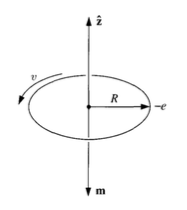
\includegraphics[width=0.94\textwidth]{./images/schematics/orbiting_electron_magnetic_dipole_moment.png}\\
    \end{center}
  \end{column}
  \begin{column}{0.65\textwidth}
     For time intervals much larger than the period of rotation T,
     we may think of the orbiting electron as a {\em steady} current I:
     \begin{equation*}
        I = \frac{q}{T} = - \frac{eu}{2\pi R}
     \end{equation*}
     where u is the electron velocity and R is the radius of its orbit (taken to be circular).
  \end{column}
\end{columns}

\vspace{0.4cm}

The {\bf magnetic dipole moment associated with that orbital motion} is:
\begin{equation*}
  \vec{m} = I \vec{S} = \Big( - \frac{eu}{2\pi R} \Big) \Big( \pi R^2 \hat{z} \Big) \Rightarrow
  \vec{m} = - \frac{1}{2} e u R \hat{z}
\end{equation*}

\end{frame}

%
%
%

\begin{frame}{Physical origin of diamagnetism}

Within an external $\vec{B}$ field, there is a significant effect on the electron orbit.

\begin{columns}
  \begin{column}{0.25\textwidth}
    \begin{center}
      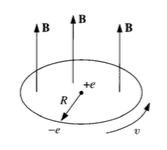
\includegraphics[width=0.90\textwidth]{./images/schematics/orbiting_electron_in_magnetic_field.png}\\
    \end{center}
  \end{column}
  \begin{column}{0.75\textwidth}
     In the absence of a $\vec{B}$ field, Coulomb's force (due to the nucleus) provides centripetal acceleration:
     \begin{equation*}
        \frac{1}{4\pi \epsilon_0} \frac{e^2}{R^2} = m_e \frac{u^2}{R}
     \end{equation*}
  \end{column}
\end{columns}
In the presence of a $\vec{B}$ field, there is an additional force $-e \Big( \vec{u} \times \vec{B} \Big)$.

Assuming (for simplicity) that $\vec{B}$ is perpendicular to the orbital plane, then:
\begin{equation*}
   \frac{1}{4\pi \epsilon_0} \frac{e^2}{R^2} + e \bar{u} B = m_e \frac{\bar{u}^2}{R} \Rightarrow
   m_e \frac{u^2}{R} + e \bar{u} B = m_e \frac{\bar{u}^2}{R} \Rightarrow
\end{equation*}
\begin{equation*}
    e \bar{u} B = \frac{m_e}{R} \Big( \bar{u}^2 - u^2 \Big) \Rightarrow
    e \bar{u} B = \frac{m_e}{R} \Big( \bar{u} + u \Big)  \Big( \bar{u} - u \Big)
\end{equation*}

\end{frame}


%
%
%

\begin{frame}{Physical origin of diamagnetism}

Assuming that the change ${\Delta}u = \bar{u} - u$ is small, so that $\bar{u} + u \approx 2u \approx 2\bar{u}$,
we can write the previous equation as:
\begin{equation*}
    e \bar{u} B = \frac{m_e}{R} \Big( \bar{u} + u \Big)  \Big( \bar{u} - u \Big) \Rightarrow
    e \cancel{\bar{u}} B = \frac{m_e}{R} 2 \cancel{\bar{u}} {\Delta}u \Rightarrow
\end{equation*}
\begin{equation*}
    {\Delta}u = \frac{eRB}{2m_e}
\end{equation*}
In the presence of a $\vec{B}$ field, the electron velocity increases by ${\Delta}u$.
This changes its magnetic dipole moment:
\begin{equation*}
  \vec{m} = - \frac{1}{2} e u R \hat{z}
\end{equation*}
The change $ {\Delta}\vec{m}$ is given by:
\begin{equation*}
    {\Delta}\vec{m} =
      - \frac{1}{2} e {\Delta}u R \hat{z} =
      - \frac{1}{2} e \Big( \frac{eRB}{2m_e} \Big) R \hat{z} \Rightarrow
    {\Delta}\vec{m} =
      - \frac{e^2 R^2}{4m_e} \vec{B}
\end{equation*}

\end{frame}
